\documentclass[9pt]{IEEEtran}

\usepackage[english]{babel}
\usepackage{graphicx}
\usepackage{epstopdf}
\usepackage{fancyhdr}
\usepackage{amsmath}
\usepackage{amsthm}
\usepackage{amssymb}
\usepackage{url}
\usepackage{array}
\usepackage{textcomp}
\usepackage{listings}
\usepackage{hyperref}
\usepackage{xcolor}
\usepackage{colortbl}
\usepackage{float}
\usepackage{gensymb}
\usepackage{longtable}
\usepackage{supertabular}
\usepackage{multicol}

\usepackage[utf8x]{inputenc}

\usepackage[T1]{fontenc}
\usepackage{lmodern}
\input{glyphtounicode}
\pdfgentounicode=1

\graphicspath{{./figures/}}
\DeclareGraphicsExtensions{.pdf,.png,.jpg,.eps}

% correct bad hyphenation here
\hyphenation{op-tical net-works semi-conduc-tor trig-gs}

% ============================================================================================

\title{\vspace{0ex}
Mathematics 2, Part 4, Homework 1}


% ============================================================================================

\begin{document}

\maketitle
\section{Nelder-Mead implementation}
\subsection*{2-D implementation}
Firstly we implemented the two dimensional version of the Nelder-Mead method
 and tested it on a simple function: 
 \[f(x, y) = x^2 + y^2 \]

 On Figure~\ref{fig:nelder_2d} we can see the convergence of the best points using 
 the 2-d implementation of the method. 

\begin{figure}[h]
    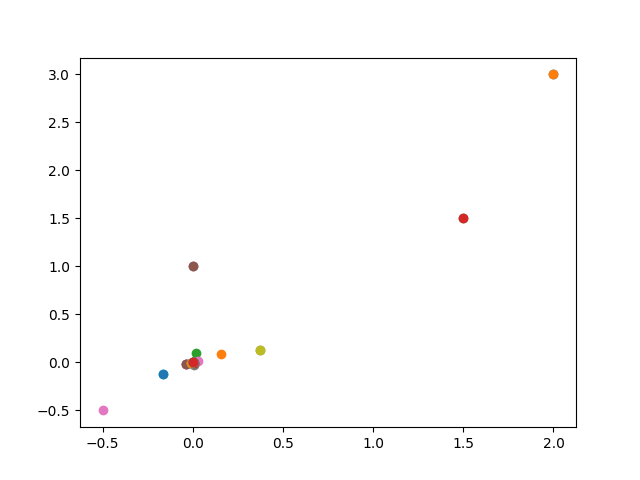
\includegraphics[width=\columnwidth]{convergence1.png}
    \caption{Convergence of the best points on a simple function for a 2-d implemntation 
    of the Nelder-Mead method}
    \label{fig:nelder_2d}
\end{figure}

\subsection*{Implementation for arbitrary dimension}
Next, we implemented Nelder-Mead for arbitrary dimensions and tested it on the 
same function. On Figure~\ref{fig:nelder} We can see that, when using the same starting points, we achieve 
the same convergence as for the previous implemtation

\begin{figure}[h]
    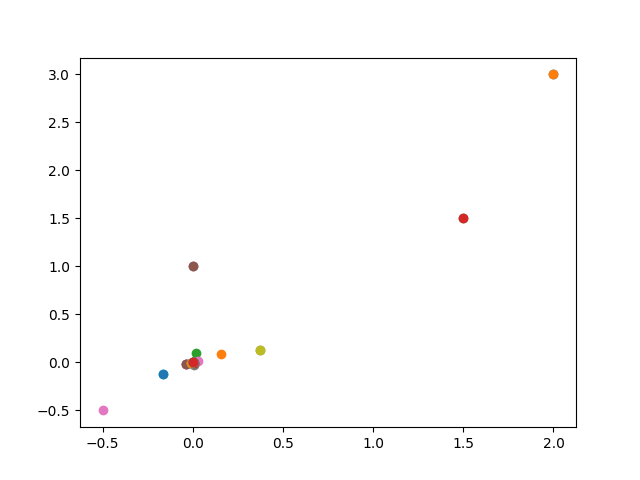
\includegraphics[width=\columnwidth]{convergence1.png}
    \caption{Convergence of the best points on a simple function 
    for the arbitrary dimensional implementation of the Nelder-Mead method}
    \label{fig:nelder}
\end{figure}

\section{Comparison of Nelder-Mead with descent methods}
We compared the implemented method with the previously implemented descent 
methods on 3 different functions. 
\subsection*{Function 1}
The first function is given as:
\[
f_1(x) = (x_0 - x_2)^2 + (2x_1 + x_2)^2 + (4x_0 - 2x_1 + x_2)^2 + x_0 + x_1
\]



\subsection*{Function 2}
\subsection*{Function 3}






\end{document}
